\chapter{Combined Fairness Definitions}
It can be desirable for models to fulfill multiple fairness definitions. However, previous works have shown that some combinations of fairness constraints are incompatible, except in degenerative cases \cite{fairness_incompatibility}. On the other hand Defrance \& De Bie \cite{max_combinations} provide a systematic analysis of the theoretical compatibility of different fairness constraints and identifies the combinations that can be satisfied simultaneously without necessarily resulting in a degenerate model. This analysis identifies twelve maximal compatible sets of constraints, consisting of five combinations of three constraints and seven combinations of two constraints. \todo{TODO: add citations + explain in detail in literary review + explain base rate of ACSIncome here + in discussion}

This chapter experimentally evaluates these theoretically compatible combinations. The aim is to determine whether the theoretical compatibility of fairness constraints translates into practical compatibility during model training, and to investigate how combining multiple constraints affects model performance.

\section{Methodology}
Models are evaluated for each of the theoretically compatible combinations of fairness definitions. An unconstrained baseline model is used as a reference to determine whether applying the fairness constraints results in an improvement in the corresponding fairness metrics and to assess the effect on predictive performance. To apply a combination of fairness metrics multiple fairrets will be used.

\subsection{Fairness Constraint Configuration}
When combining two fairness metrics, their individual losses are calculated separately and summed to form the combined fairness loss. Because each fairret using the same strength can influence a model at a different rate, each metric is assigned a separate strength parameter for each combination.

Finding suitable strengths is non-trivial because increasing the strength of one constraint can affect the value of the another metric. Improving one metric may therefore come at the expense of the another. To find suitable configurations, an initial set of constraint strengths is selected and iteratively adjusted according as follows.
As long as the model does not perform notably better than the baseline for the fairness combination, the weakest performing metric has its strength increased until it does perform notably better than the baseline model. If it does, the combination is deemed satisfiable and the strengths will be used for evaluation. If the model performance drops so low it no longer is meaningful, the combination is deemed unsatisfiable using this method.

\subsection{Evaluation}
After suitable constraint strengths have been identified, the configurations are evaluated using multiple independent training runs. For each run, a model is first trained using the unconstrained baseline configuration. The final training steps are then performed with the selected fairness constraints added to the objective.

For each resulting model, the relevant fairness metrics and predictive performance are recorded. These results are then compared with the unconstrained baseline. This makes it possible to assess both whether the theoretically compatible combinations improve the intended fairness metrics in practice and what effect this has on predictive performance.

\section{Results}
For each fairness combination, a fairness strength configuration was found and test runs were performed to evaluate the performance and fairness violations. All scores can be found in table \ref{table:combined} below, the relevant metrics are highlighted per combination. 
Figures \ref{fig:pair1} up to \ref{fig:pair21} visualise this data for each pair of constraints, to compare against the baseline and single constraint models. Figures \ref{fig:triple1} up to \ref{fig:triple5} do this too for each trio of constraints.

Reviewing these graphs shows in nearly all cases the combinations of fairness metrics could be substantially improved. The exceptions for this are PP-ACC \ref{fig:PP-ACC} and EO-TE \ref{fig:EO-TE}. This is because of poor tuning of the fairness strengths, as these aren't maximal fairness combinations, PP-FOR-ACC \ref{fig:PP-FOR-ACC} and EO-PP-TE \ref{fig:EO-PP-TE} show these pairs can be substantially satisfied.

The AUROC scores stay in an acceptable range, however it's clear not every combination is affected equally. ACC-TE improved the violations significantly while achieving an AUROC score above 0.89. On the other hand EO-FOR drops to an AUROC of 0.77 for comparable improvements to the violations.
\todo{TODO: optional, Check with base rates diffs if this can be explained with min max ranges in MAX paper}

The pairs EO-PP, EO-TE, PP-TE, PE-FOR, PE-TE and FOR-TE are all special cases of non-maximal combinations. These have the property of satisfying their respective maximal trio of constraints EO-PP-TE and PE-FOR-TE \cite{max_combinations}.
This is present in the results of table \ref{table:combined} for PE-FOR, EO-PP and PE-TE. As for EO-TE, PP-TE and FOR-TE the opposite is true, the supposed third constraint performs worse than the baseline. When tuning FOR-TE with stronger fairness constraints, the third constraint PE does improve substantially. Figures \ref{fig:forte} show the PE violation initially gets worse, but as the FOR violation improves further while TE remains stable and low, PE starts improving as well. EO-TE and PP-TE showed similar training behaviour.

% \newlength\q
% \setlength\q{\dimexpr .5\textwidth -2\tabcolsep}
\begin{table}[htbp]{}
    \resizebox{\textwidth}{!}{
    \begin{tabular}{|l|r|r|r|r|r|r|r|r|}
    \hline
    Constraints & AUROC & DP & EO & PE & PP & FOR & ACC & TE \\
    \hline
    none & 0.897521 & 0.111902 & 0.020183 & 0.056207 & 0.084910 & 0.195691 & 0.016241 & 0.182619 
    \\\hline
    DP & 0.886538 & \textbf{0.011279} & 0.048058 & 0.104905 & 0.120792 & 0.256330 & 0.004025 & 0.517258 \\
    EO & 0.896274 & 0.088830 & \textbf{0.001208} & 0.023399 & 0.088610 & 0.213870 & 0.018497 & 0.251354 \\
    PE & 0.896630 & 0.094250 & 0.010807 & \textbf{0.022783} & 0.094159 & 0.199665 & 0.013824 & 0.233879 \\
    PP & 0.897362 & 0.126060 & 0.026220 & 0.087097 & \textbf{0.075816} & 0.195199 & 0.019967 & 0.149043 \\
    FOR & 0.896962 & 0.129998 & 0.040683 & 0.075827 & 0.085420 & \textbf{0.176882} & 0.014130 & 0.136654 \\
    ACC & 0.890181 & 0.120685 & 0.049211 & 0.063545 & 0.103131 & 0.162940 & \textbf{0.005009} & 0.124801 \\
    TE & 0.895972 & 0.153835 & 0.053813 & 0.127726 & 0.072527 & 0.173833 & 0.019276 & \textbf{0.071930} \\
    \hline
    DP-EO-PE & 0.892701 & \textbf{0.056369} & \textbf{0.003284} & \textbf{0.014502} & 0.118137 & 0.206739 & 0.006965 & 0.302611 \\
    EO-PE-ACC & 0.894609 & 0.078604 & \textbf{0.007057} & \textbf{0.004200} & 0.106162 & 0.202118 & \textbf{0.005595} & 0.260853 \\
    EO-PP-TE & 0.873637 & 0.144380 & \textbf{0.007387} & 0.201188 & \textbf{0.037768} & 0.279536 & 0.046325 & \textbf{0.067978} \\
    PE-FOR-TE & 0.846189 & 0.124984 & 0.121221 & \textbf{0.028727} & 0.167015 & \textbf{0.063446} & 0.030082 & \textbf{0.040522} \\
    PP-FOR-ACC & 0.867213 & 0.316549 & 0.202012 & 0.367275 & \textbf{0.031530} & \textbf{0.070262} & \textbf{0.013325} & 0.471879 \\
    DP-PP & 0.846814 & \textbf{0.023696} & 0.147311 & 0.086615 & \textbf{0.025289} & 0.282993 & 0.081047 & 0.293131 \\
    DP-FOR & 0.806854 & \textbf{0.014641} & 0.079795 & 0.140756 & 0.225417 & \textbf{0.069791} & 0.067183 & 0.359281 \\
    DP-ACC & 0.886812 & \textbf{0.020757} & 0.035932 & 0.092130 & 0.122552 & 0.235755 & \textbf{0.004752} & 0.468474 \\
    DP-TE & 0.856222 & \textbf{0.053880} & 0.040425 & 0.020361 & 0.158774 & 0.080615 & 0.058167 & \textbf{0.046628} \\
    EO-FOR & 0.771971 & 0.023146 & \textbf{0.006506} & 0.065255 & 0.194608 & \textbf{0.044103} & 0.145780 & 0.326048 \\
    PE-PP & 0.846899 & 0.047570 & 0.223475 & \textbf{0.014613} & \textbf{0.031319} & 0.208129 & 0.099684 & 0.336185 \\
    ACC-TE & 0.890142 & 0.153551 & 0.072801 & 0.116927 & 0.091445 & 0.142647 & \textbf{0.006943} & \textbf{0.027015} \\
    \hline
    DP-EO & 0.885103 & \textbf{0.030340} & \textbf{0.006478} & 0.060875 & 0.139072 & 0.197470 & 0.004375 & 0.371632 \\
    DP-PE & 0.889531 & \textbf{0.040468} & 0.042151 & \textbf{0.017778} & 0.099151 & 0.249565 & 0.021750 & 0.362127 \\
    EO-PE & 0.895874 & 0.082070 & \textbf{0.001044} & \textbf{0.009375} & 0.095469 & 0.211793 & 0.015154 & 0.268505 \\
    EO-ACC & 0.894422 & 0.075213 & \textbf{0.003890} & 0.005198 & 0.106600 & 0.205398 & \textbf{0.004973} & 0.278370 \\
    EO-TE* & 0.880410 & 0.115452 & \textbf{0.004274} & 0.138552 & 0.066141 & \textbf{0.256128} & 0.035520 & \textbf{0.137928} \\
    PE-ACC & 0.893884 & 0.092378 & 0.023437 & \textbf{0.022904} & 0.107566 & 0.183974 & \textbf{0.003287} & 0.207968 \\
    PE-TE* & 0.854810 & 0.079303 & 0.072894 & \textbf{0.018147} & 0.164794 & \textbf{0.078869} & 0.041809 & \textbf{0.068125} \\
    PP-FOR & 0.863021 & 0.323068 & 0.197308 & 0.403291 & \textbf{0.016471} & \textbf{0.076303} & 0.020773 & 0.565290 \\
    PP-ACC & 0.876104 & 0.294753 & 0.177746 & 0.326858 & \textbf{0.032936} & 0.098818 & \textbf{0.014933} & 0.311299 \\
    FOR-ACC & 0.866339 & 0.246898 & 0.170520 & 0.220132 & 0.086449 & \textbf{0.076305} & \textbf{0.004357} & 0.202295 \\
    PP-TE* & 0.879404 & 0.194886 & \textbf{0.051028} & 0.264834 & \textbf{0.022367} & 0.208932 & 0.042277 & \textbf{0.077580} \\
    EO-PP* & 0.881559 & 0.134423 & \textbf{0.005534} & 0.174653 & \textbf{0.047063} & 0.269218 & 0.038653 & \textbf{0.098857} \\
    PE-FOR* & 0.847975 & 0.146495 & 0.142830 & \textbf{0.030366} & 0.167007 & \textbf{0.075402} & 0.021601 & \textbf{0.059938} \\
    FOR-TE* & 0.855044 & 0.165001 & 0.131718 & \textbf{0.083057} & 0.137507 & \textbf{0.060540} & 0.017420 & \textbf{0.035933} \\\hline
    \end{tabular}}
    \caption{Average performance and fairness violations of all fairness combinations}
    \label{table:combined}
\end{table}
\begin{figure}[htbp]
    \centering
    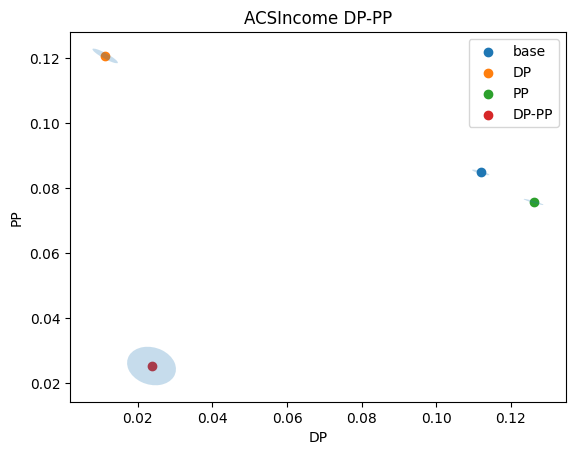
\includegraphics[width=0.8\textwidth]{assets/combined/ACSIncome_DP-PP.png}
    \caption{Violation measures of DP and PP for an unconstrained baseline model, single constrained models and a combined constrained model. Averages were calculated from 5 samples runs.}
    \label{fig:pair1}
\end{figure}



\begin{figure}[htbp]
    \centering
    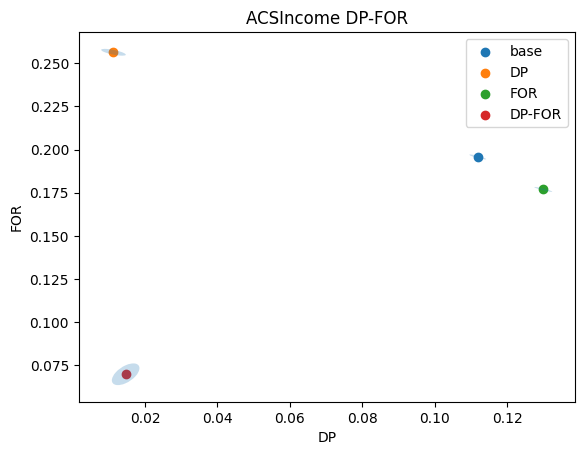
\includegraphics[width=0.8\textwidth]{assets/combined/ACSIncome_DP-FOR.png}
    \caption{Violation measures of DP and FOR for an unconstrained baseline model, single constrained models and a combined constrained model. Averages were calculated from 5 samples runs.}
\end{figure}
    

\begin{figure}[htbp]
    \centering
    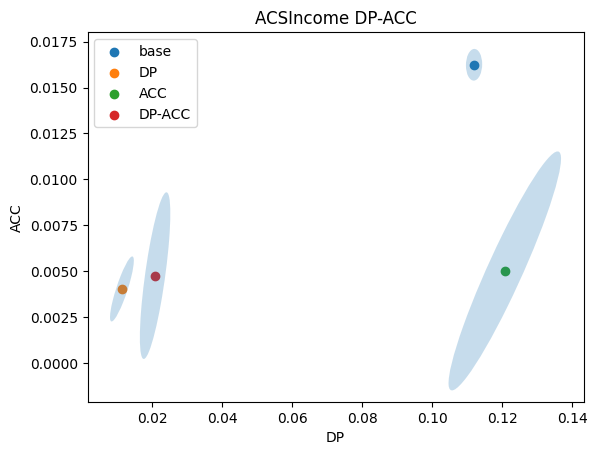
\includegraphics[width=0.8\textwidth]{assets/combined/ACSIncome_DP-ACC.png}
    \caption{Violation measures of DP and ACC for an unconstrained baseline model, single constrained models and a combined constrained model. Averages were calculated from 5 samples runs.}
\end{figure}
    

\begin{figure}[htbp]
    \centering
    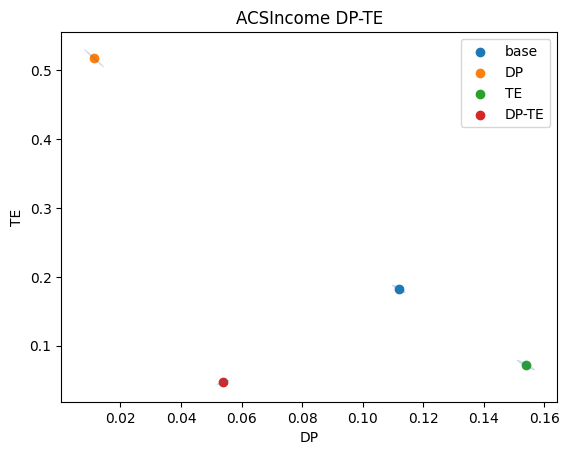
\includegraphics[width=0.8\textwidth]{assets/combined/ACSIncome_DP-TE.png}
    \caption{Violation measures of DP and TE for an unconstrained baseline model, single constrained models and a combined constrained model. Averages were calculated from 5 samples runs.}
\end{figure}
    

\begin{figure}[htbp]
    \centering
    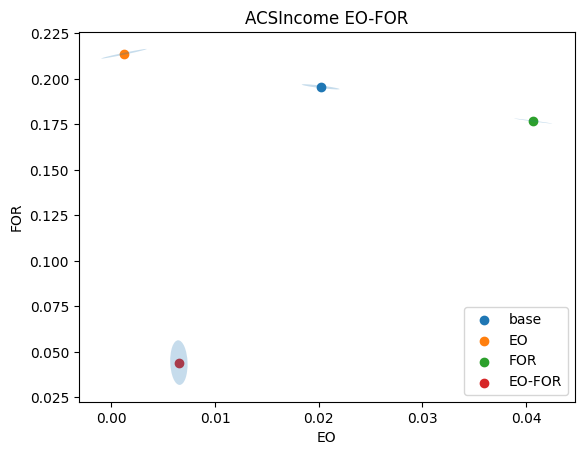
\includegraphics[width=0.8\textwidth]{assets/combined/ACSIncome_EO-FOR.png}
    \caption{Violation measures of EO and FOR for an unconstrained baseline model, single constrained models and a combined constrained model. Averages were calculated from 5 samples runs.}
\end{figure}
    

\begin{figure}[htbp]
    \centering
    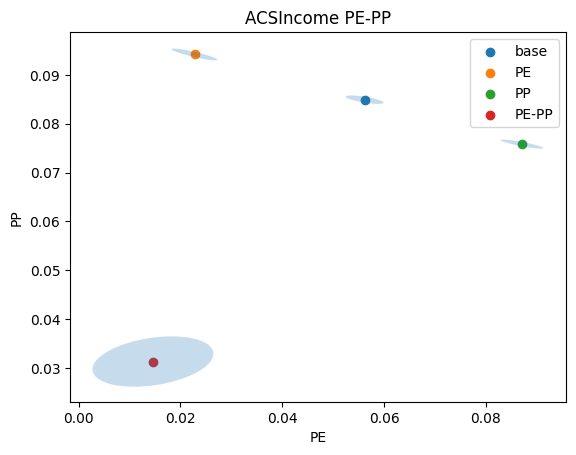
\includegraphics[width=0.8\textwidth]{assets/combined/ACSIncome_PE-PP.png}
    \caption{Violation measures of PE and PP for an unconstrained baseline model, single constrained models and a combined constrained model. Averages were calculated from 5 samples runs.}
\end{figure}
    

\begin{figure}[htbp]
    \centering
    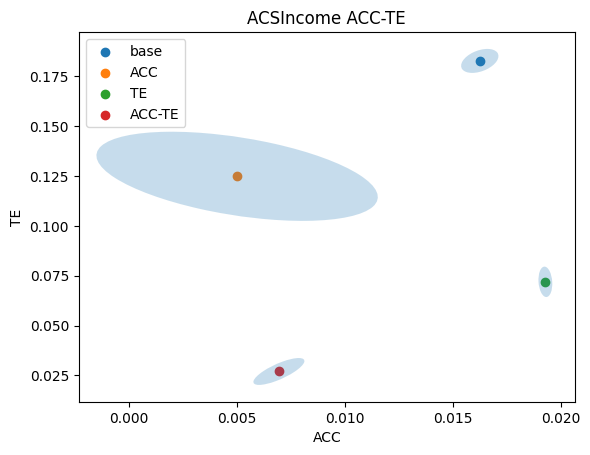
\includegraphics[width=0.8\textwidth]{assets/combined/ACSIncome_ACC-TE.png}
    \caption{Violation measures of ACC and TE for an unconstrained baseline model, single constrained models and a combined constrained model. Averages were calculated from 5 samples runs.}
\end{figure}
    

\begin{figure}[htbp]
    \centering
    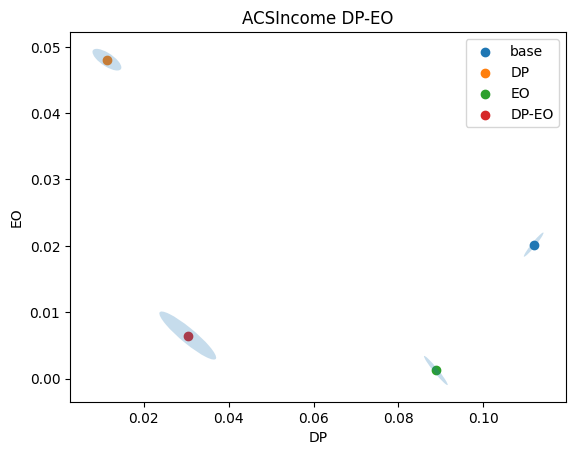
\includegraphics[width=0.8\textwidth]{assets/combined/ACSIncome_DP-EO.png}
    \caption{Violation measures of DP and EO for an unconstrained baseline model, single constrained models and a combined constrained model. Averages were calculated from 5 samples runs.}
\end{figure}
    

\begin{figure}[htbp]
    \centering
    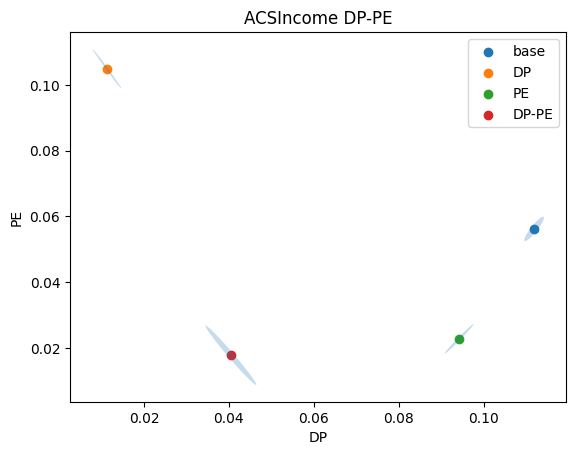
\includegraphics[width=0.8\textwidth]{assets/combined/ACSIncome_DP-PE.png}
    \caption{Violation measures of DP and PE for an unconstrained baseline model, single constrained models and a combined constrained model. Averages were calculated from 5 samples runs.}
\end{figure}
    

\begin{figure}[htbp]
    \centering
    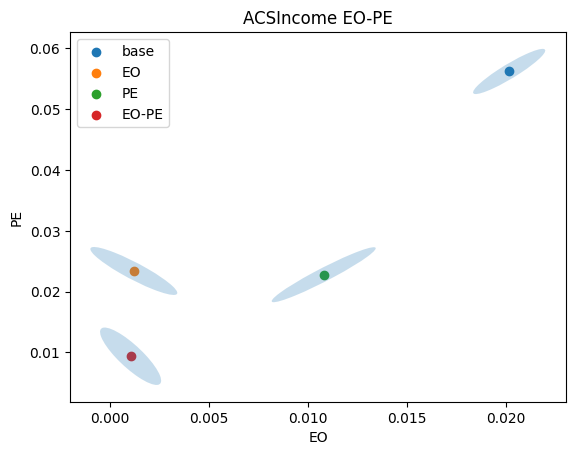
\includegraphics[width=0.8\textwidth]{assets/combined/ACSIncome_EO-PE.png}
    \caption{Violation measures of EO and PE for an unconstrained baseline model, single constrained models and a combined constrained model. Averages were calculated from 5 samples runs.}
\end{figure}
    

\begin{figure}[htbp]
    \centering
    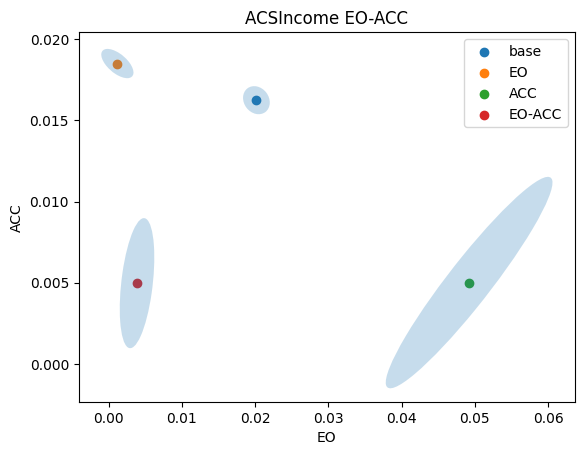
\includegraphics[width=0.8\textwidth]{assets/combined/ACSIncome_EO-ACC.png}
    \caption{Violation measures of EO and ACC for an unconstrained baseline model, single constrained models and a combined constrained model. Averages were calculated from 5 samples runs.}
\end{figure}
    

\begin{figure}[htbp]
    \centering
    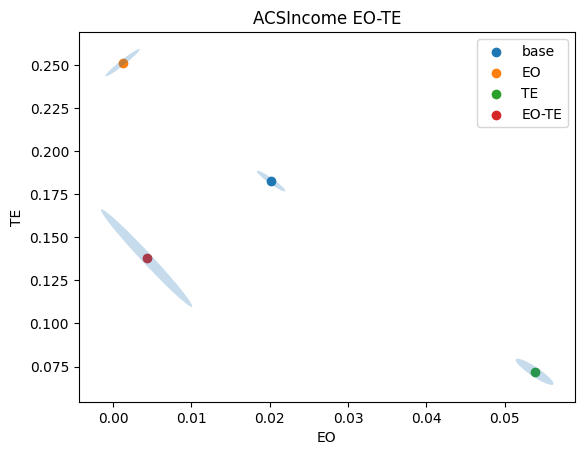
\includegraphics[width=0.8\textwidth]{assets/combined/ACSIncome_EO-TE.png}
    \caption{Violation measures of EO and TE for an unconstrained baseline model, single constrained models and a combined constrained model. Averages were calculated from 5 samples runs.}
    \label{fig:EO-TE}
\end{figure}
    

\begin{figure}[htbp]
    \centering
    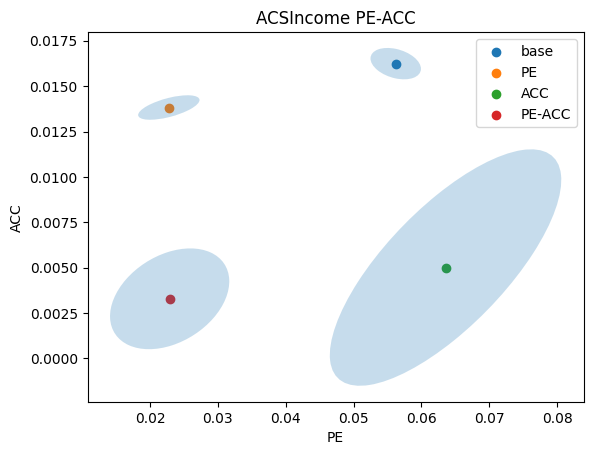
\includegraphics[width=0.8\textwidth]{assets/combined/ACSIncome_PE-ACC.png}
    \caption{Violation measures of PE and ACC for an unconstrained baseline model, single constrained models and a combined constrained model. Averages were calculated from 5 samples runs.}
\end{figure}
    

\begin{figure}[htbp]
    \centering
    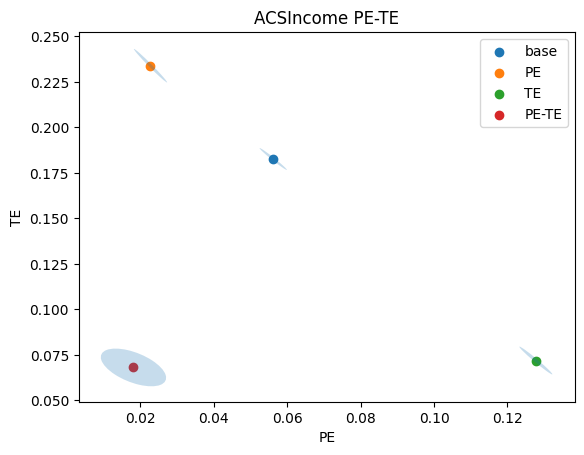
\includegraphics[width=0.8\textwidth]{assets/combined/ACSIncome_PE-TE.png}
    \caption{Violation measures of PE and TE for an unconstrained baseline model, single constrained models and a combined constrained model. Averages were calculated from 5 samples runs.}
\end{figure}
    

\begin{figure}[htbp]
    \centering
    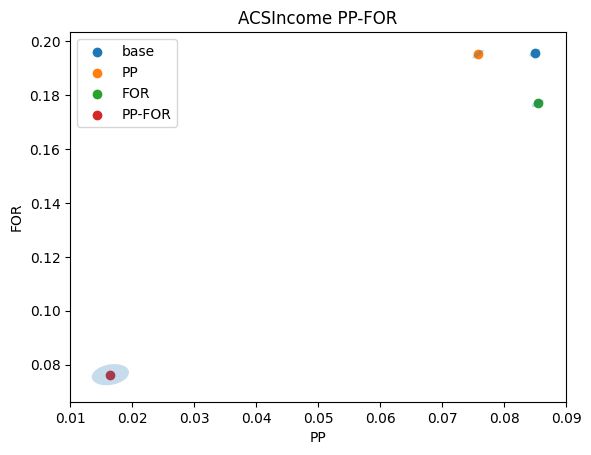
\includegraphics[width=0.8\textwidth]{assets/combined/ACSIncome_PP-FOR.png}
    \caption{Violation measures of PP and FOR for an unconstrained baseline model, single constrained models and a combined constrained model. Averages were calculated from 5 samples runs.}
\end{figure}
    

\begin{figure}[htbp]
    \centering
    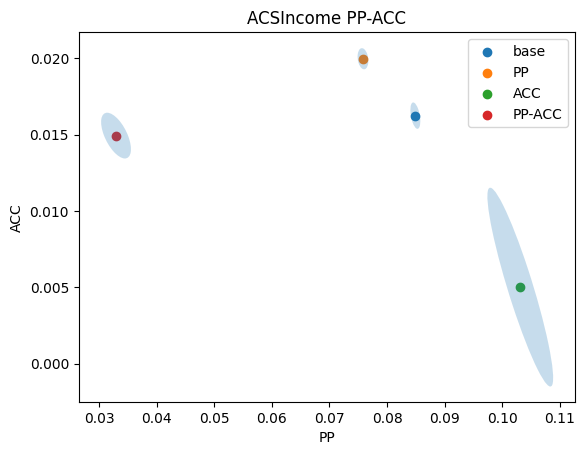
\includegraphics[width=0.8\textwidth]{assets/combined/ACSIncome_PP-ACC.png}
    \caption{Violation measures of PP and ACC for an unconstrained baseline model, single constrained models and a combined constrained model. Averages were calculated from 5 samples runs.}
    \label{fig:PP-ACC}
\end{figure}
    

\begin{figure}[htbp]
    \centering
    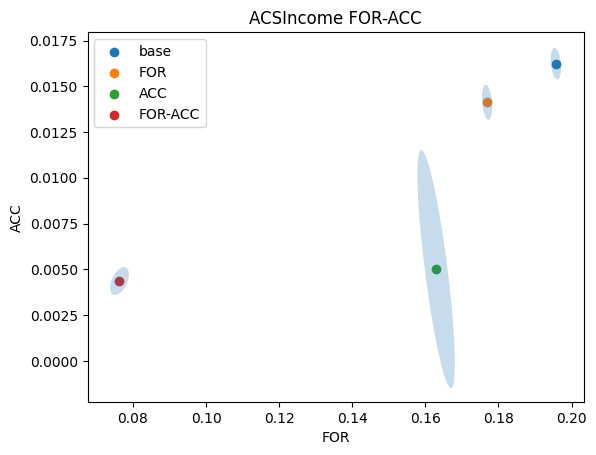
\includegraphics[width=0.8\textwidth]{assets/combined/ACSIncome_FOR-ACC.png}
    \caption{Violation measures of FOR and ACC for an unconstrained baseline model, single constrained models and a combined constrained model. Averages were calculated from 5 samples runs.}
\end{figure}
    

\begin{figure}[htbp]
    \centering
    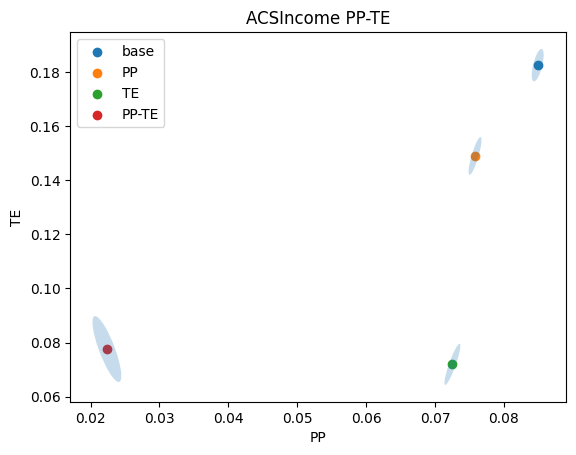
\includegraphics[width=0.8\textwidth]{assets/combined/ACSIncome_PP-TE.png}
    \caption{Violation measures of PP and TE for an unconstrained baseline model, single constrained models and a combined constrained model. Averages were calculated from 5 samples runs.}
\end{figure}
    

\begin{figure}[htbp]
    \centering
    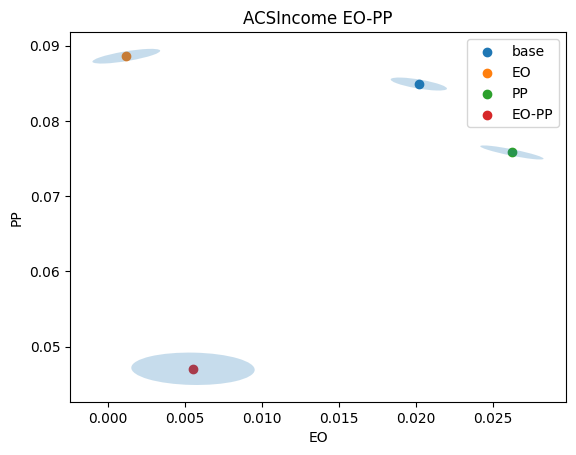
\includegraphics[width=0.8\textwidth]{assets/combined/ACSIncome_EO-PP.png}
    \caption{Violation measures of EO and PP for an unconstrained baseline model, single constrained models and a combined constrained model. Averages were calculated from 5 samples runs.}
\end{figure}
    

\begin{figure}[htbp]
    \centering
    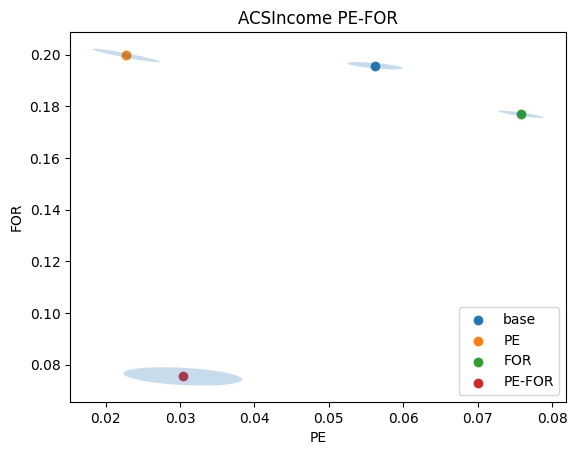
\includegraphics[width=0.8\textwidth]{assets/combined/ACSIncome_PE-FOR.png}
    \caption{Violation measures of PE and FOR for an unconstrained baseline model, single constrained models and a combined constrained model. Averages were calculated from 5 samples runs.}
\end{figure}
    

\begin{figure}[htbp]
    \centering
    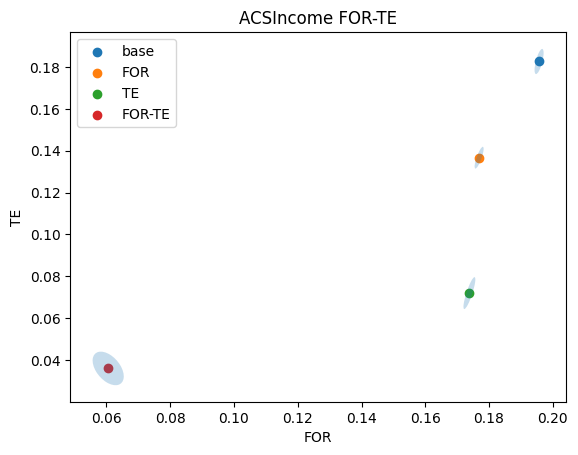
\includegraphics[width=0.8\textwidth]{assets/combined/ACSIncome_FOR-TE.png}
    \caption{Violation measures of FOR and TE for an unconstrained baseline model, single constrained models and a combined constrained model. Averages were calculated from 5 samples runs.}
    \label{fig:pair21}
\end{figure}

\begin{figure}[htbp]
    \centering
    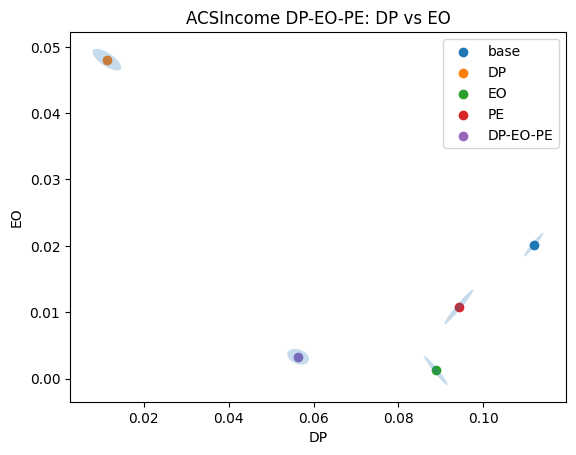
\includegraphics[width=0.45\textwidth]{assets/combined/ACSIncome_DP-EO-PE_DP-EO.png}
    \hfill
    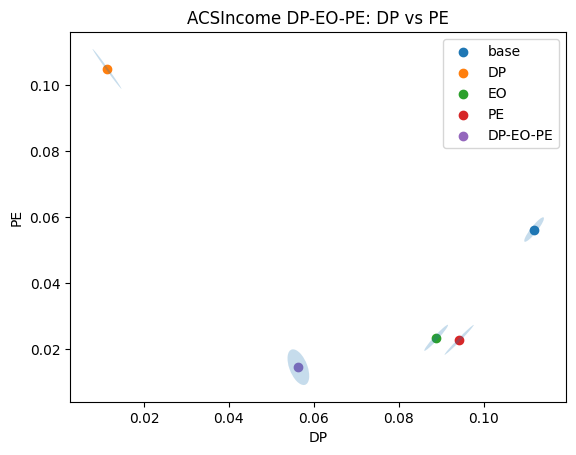
\includegraphics[width=0.45\textwidth]{assets/combined/ACSIncome_DP-EO-PE_DP-PE.png}
    \hfill
    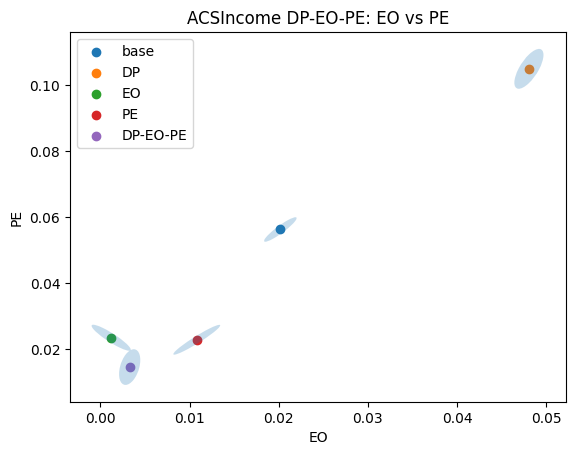
\includegraphics[width=0.45\textwidth]{assets/combined/ACSIncome_DP-EO-PE_EO-PE.png}
    \caption{Violation measures of DP, EO and PE for an unconstrained baseline model, single constrained models and a combined constrained model. Averages were calculated from 5 samples runs.}
    \label{fig:triple1}
\end{figure}
        
\begin{figure}[htbp]
    \centering
    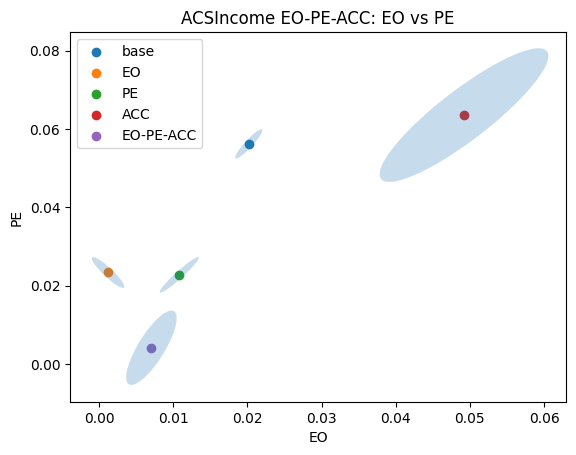
\includegraphics[width=0.45\textwidth]{assets/combined/ACSIncome_EO-PE-ACC_EO-PE.png}
    \hfill
    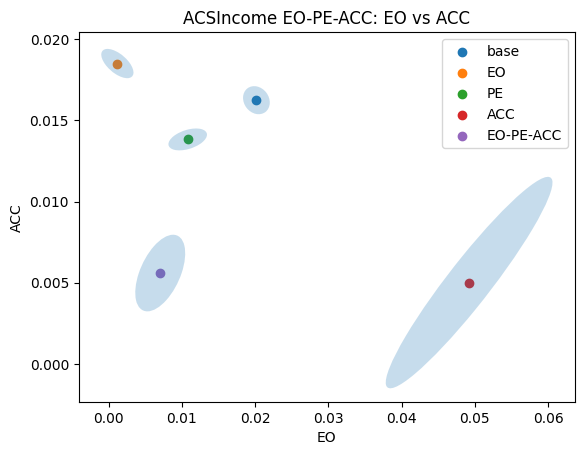
\includegraphics[width=0.45\textwidth]{assets/combined/ACSIncome_EO-PE-ACC_EO-ACC.png}
    \hfill
    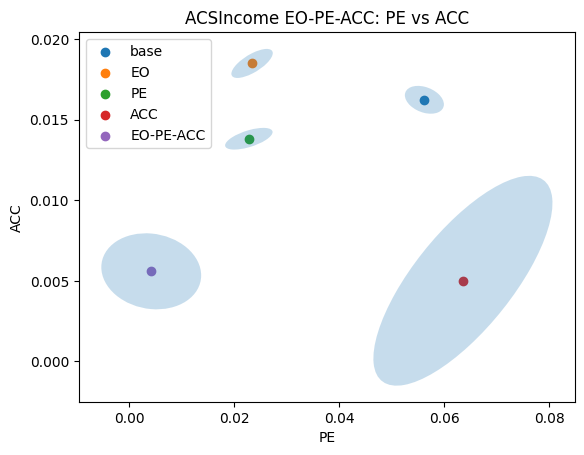
\includegraphics[width=0.45\textwidth]{assets/combined/ACSIncome_EO-PE-ACC_PE-ACC.png}
    \caption{Violation measures of EO, PE and ACC for an unconstrained baseline model, single constrained models and a combined constrained model. Averages were calculated from 5 samples runs.}
\end{figure}
        
\begin{figure}[htbp]
    \centering
    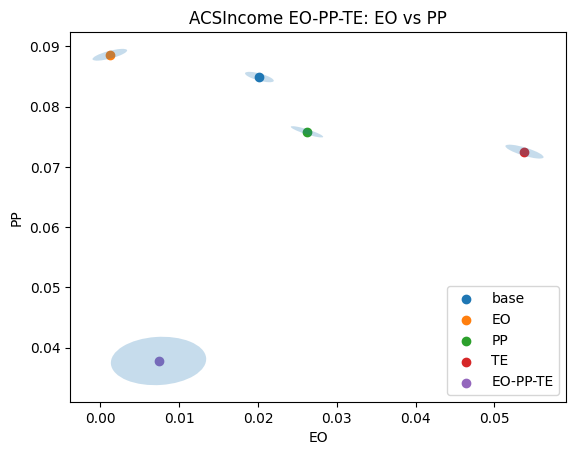
\includegraphics[width=0.45\textwidth]{assets/combined/ACSIncome_EO-PP-TE_EO-PP.png}
    \hfill
    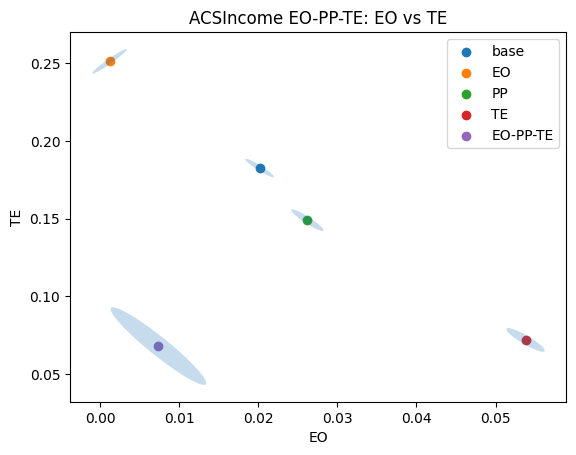
\includegraphics[width=0.45\textwidth]{assets/combined/ACSIncome_EO-PP-TE_EO-TE.png}
    \hfill
    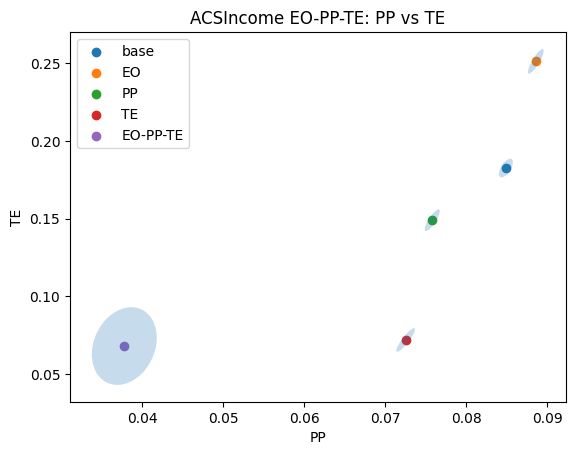
\includegraphics[width=0.45\textwidth]{assets/combined/ACSIncome_EO-PP-TE_PP-TE.png}
    \caption{Violation measures of EO, PP and TE for an unconstrained baseline model, single constrained models and a combined constrained model. Averages were calculated from 5 samples runs.}
    \label{fig:EO-PP-TE}
\end{figure}
        
\begin{figure}[htbp]
    \centering
    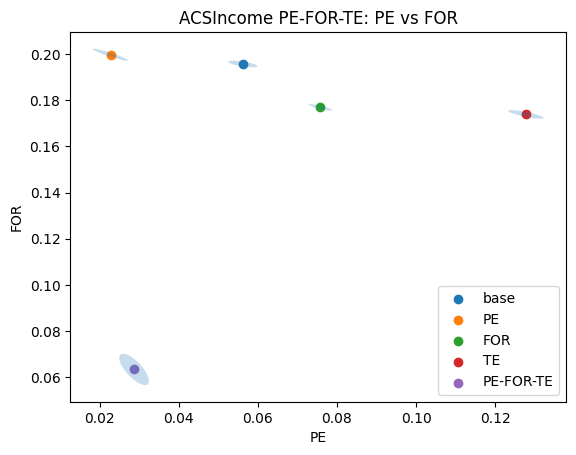
\includegraphics[width=0.45\textwidth]{assets/combined/ACSIncome_PE-FOR-TE_PE-FOR.png}
    \hfill
    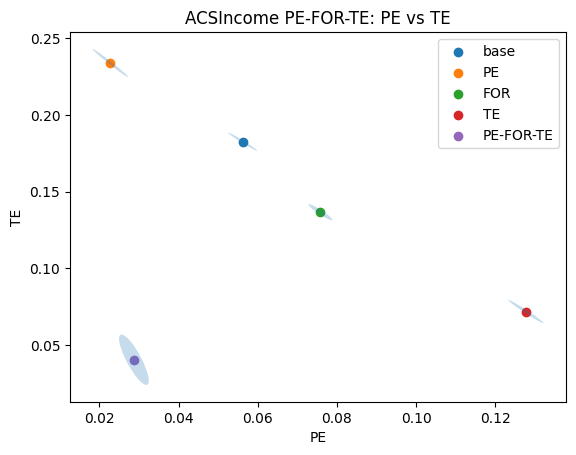
\includegraphics[width=0.45\textwidth]{assets/combined/ACSIncome_PE-FOR-TE_PE-TE.png}
    \hfill
    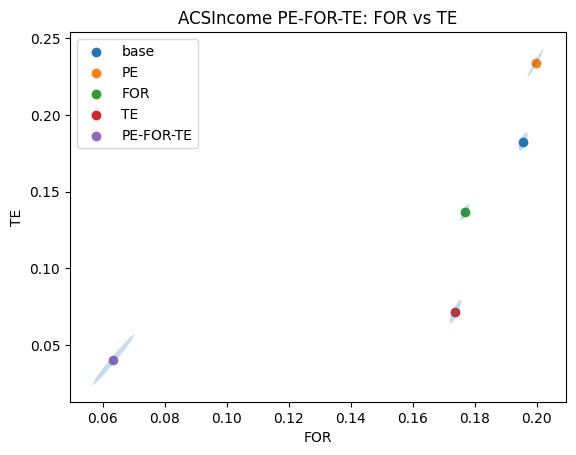
\includegraphics[width=0.45\textwidth]{assets/combined/ACSIncome_PE-FOR-TE_FOR-TE.png}
    \caption{Violation measures of PE, FOR and TE for an unconstrained baseline model, single constrained models and a combined constrained model. Averages were calculated from 5 samples runs.}
\end{figure}
        
\begin{figure}[htbp]
    \centering
    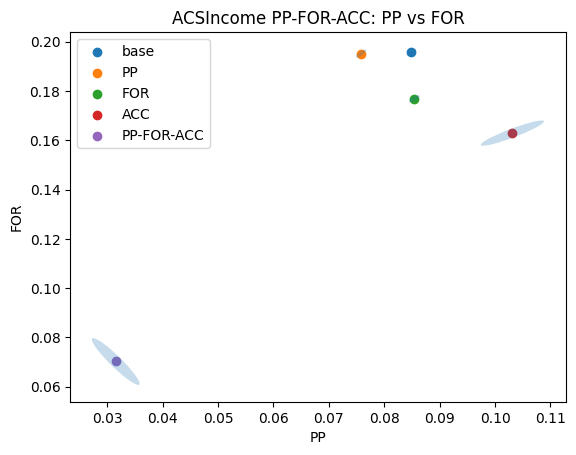
\includegraphics[width=0.45\textwidth]{assets/combined/ACSIncome_PP-FOR-ACC_PP-FOR.png}
    \hfill
    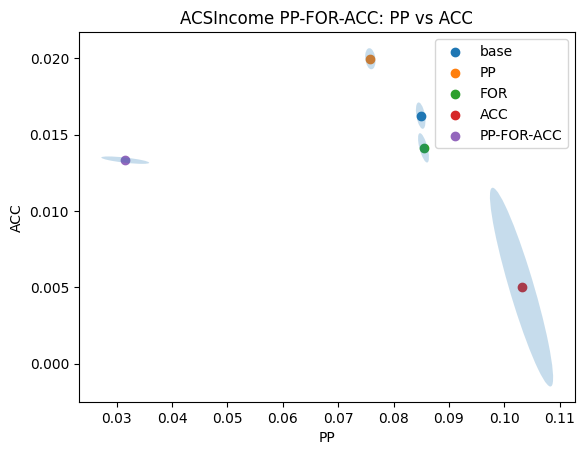
\includegraphics[width=0.45\textwidth]{assets/combined/ACSIncome_PP-FOR-ACC_PP-ACC.png}
    \hfill
    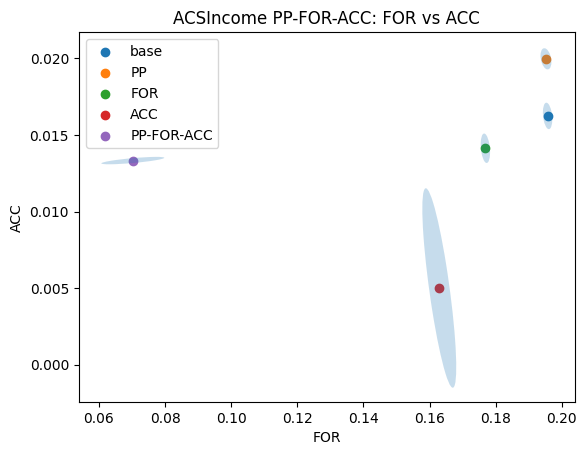
\includegraphics[width=0.45\textwidth]{assets/combined/ACSIncome_PP-FOR-ACC_FOR-ACC.png}
    \caption{Violation measures of PP, FOR and ACC for an unconstrained baseline model, single constrained models and a combined constrained model. Averages were calculated from 5 samples runs.}
    \label{fig:triple5}
    \label{fig:PP-FOR-ACC}
\end{figure}
\begin{figure}[htbp]
    \centering
    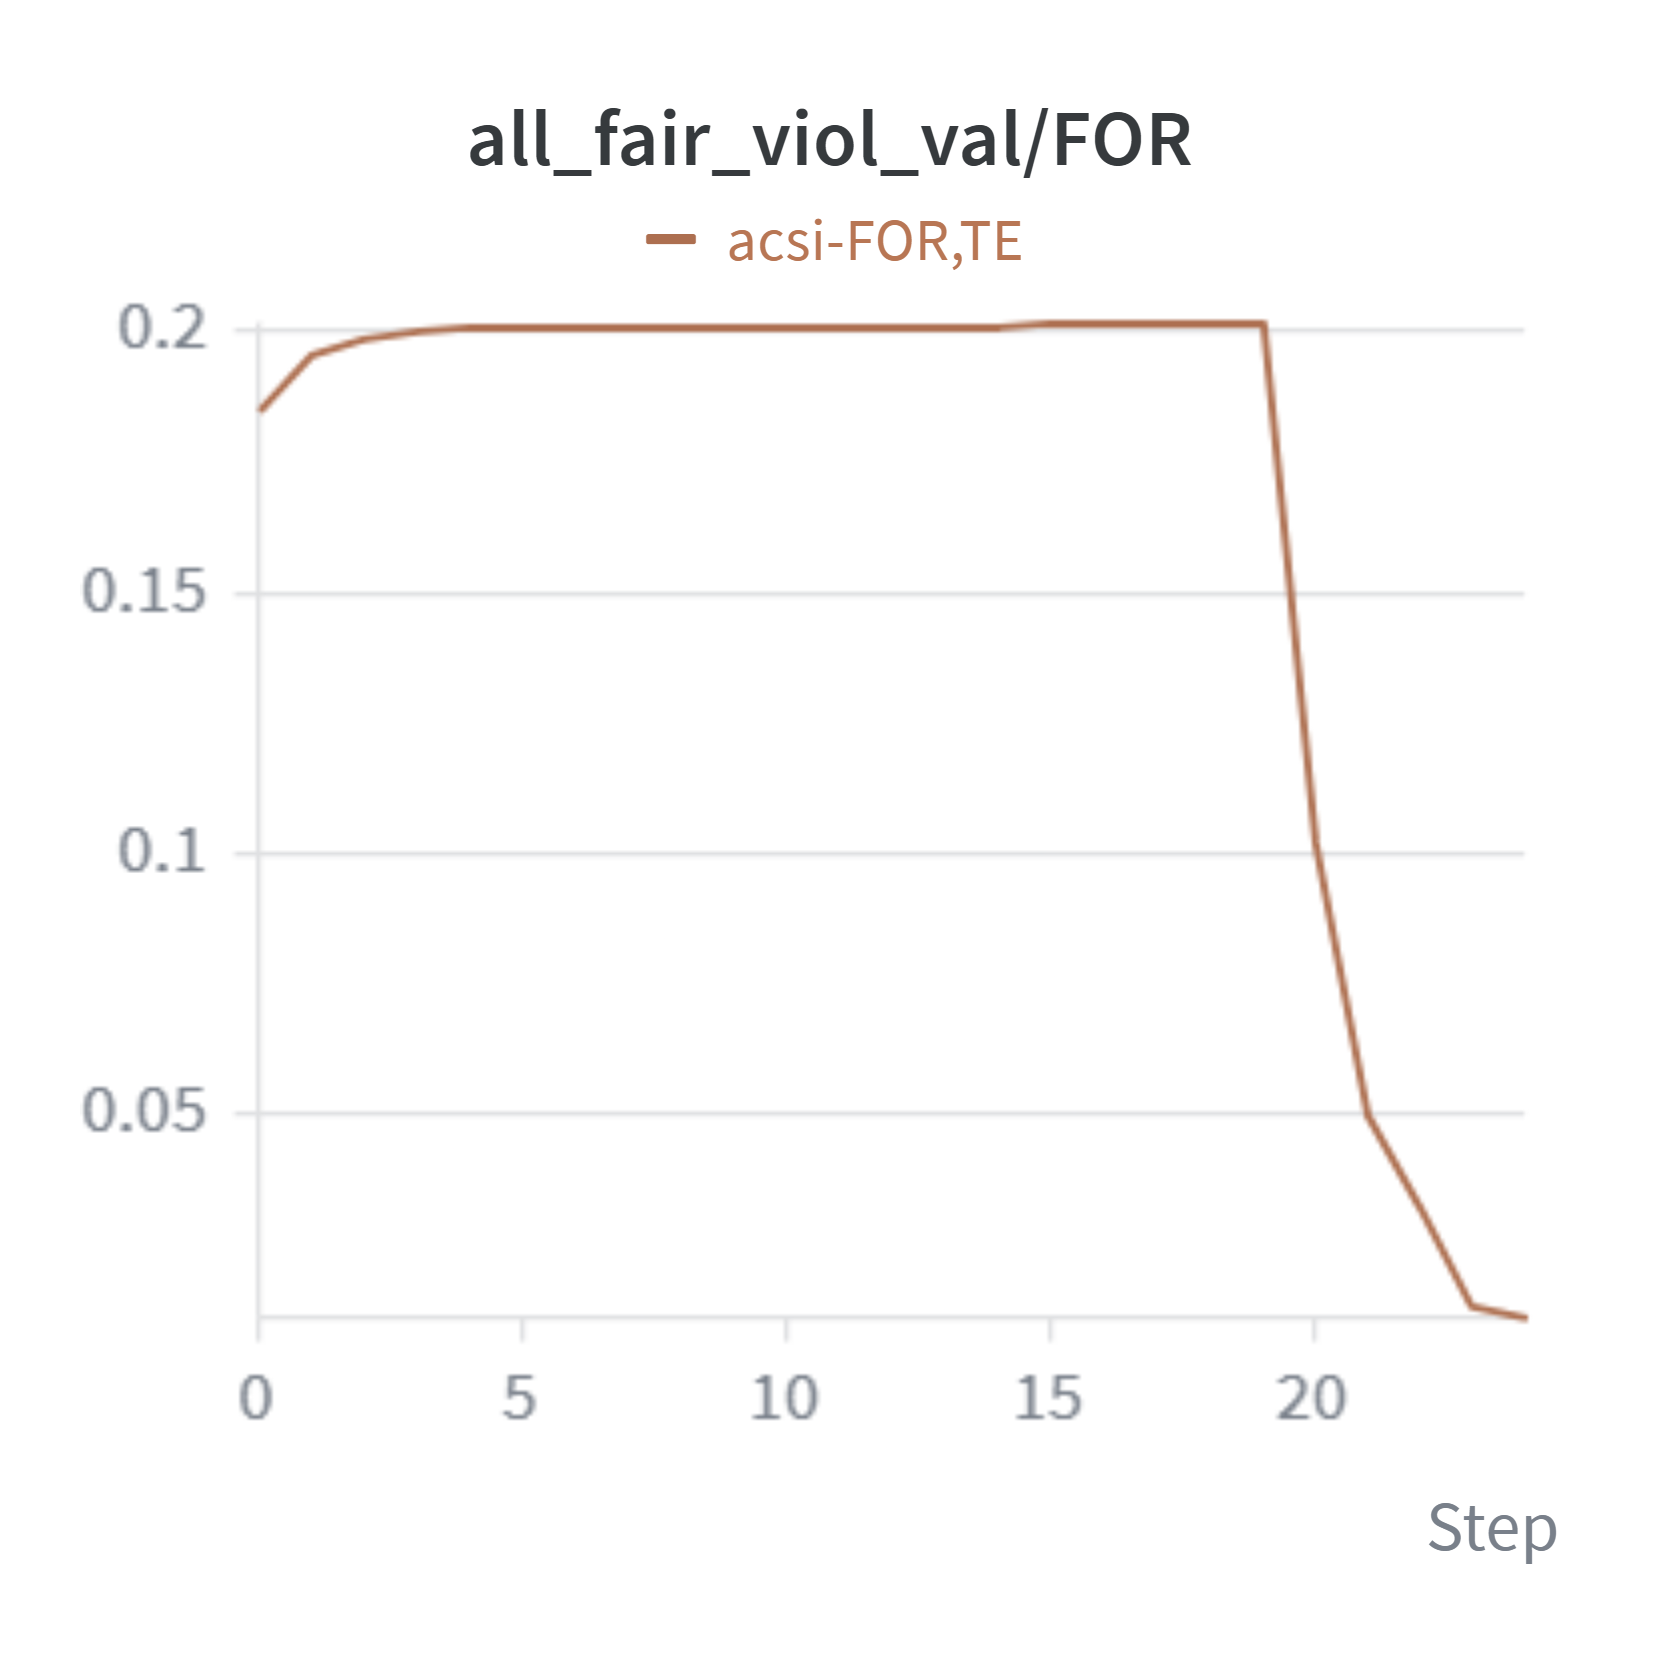
\includegraphics[width=0.45\textwidth]{assets/combined/ACSIncome_FORTE1.png}
    \hfill
    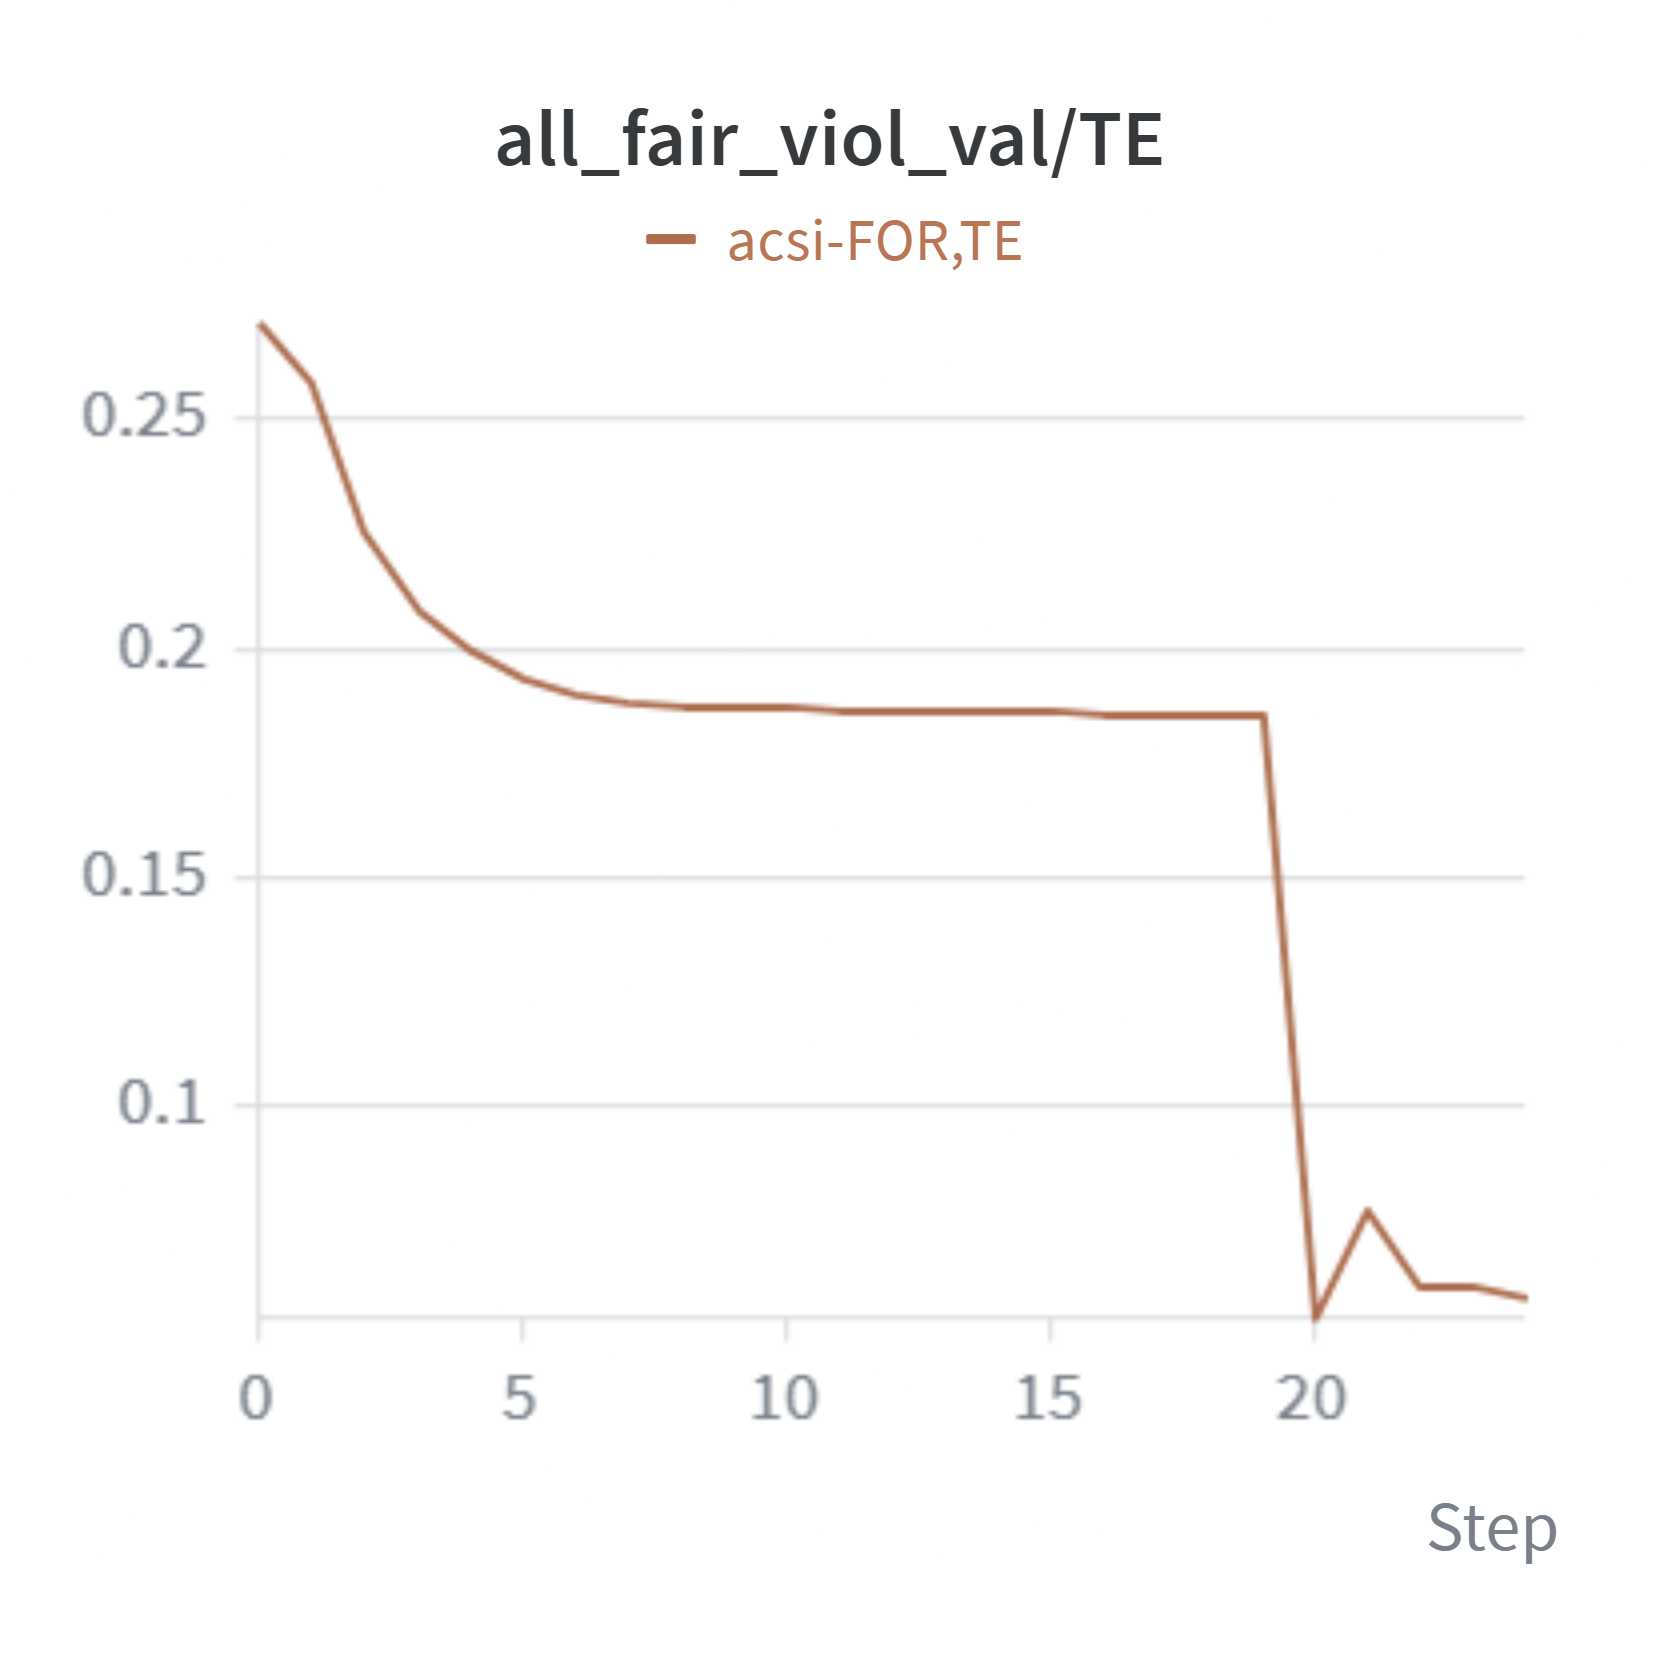
\includegraphics[width=0.45\textwidth]{assets/combined/ACSIncome_FORTE2.png}
    \hfill
    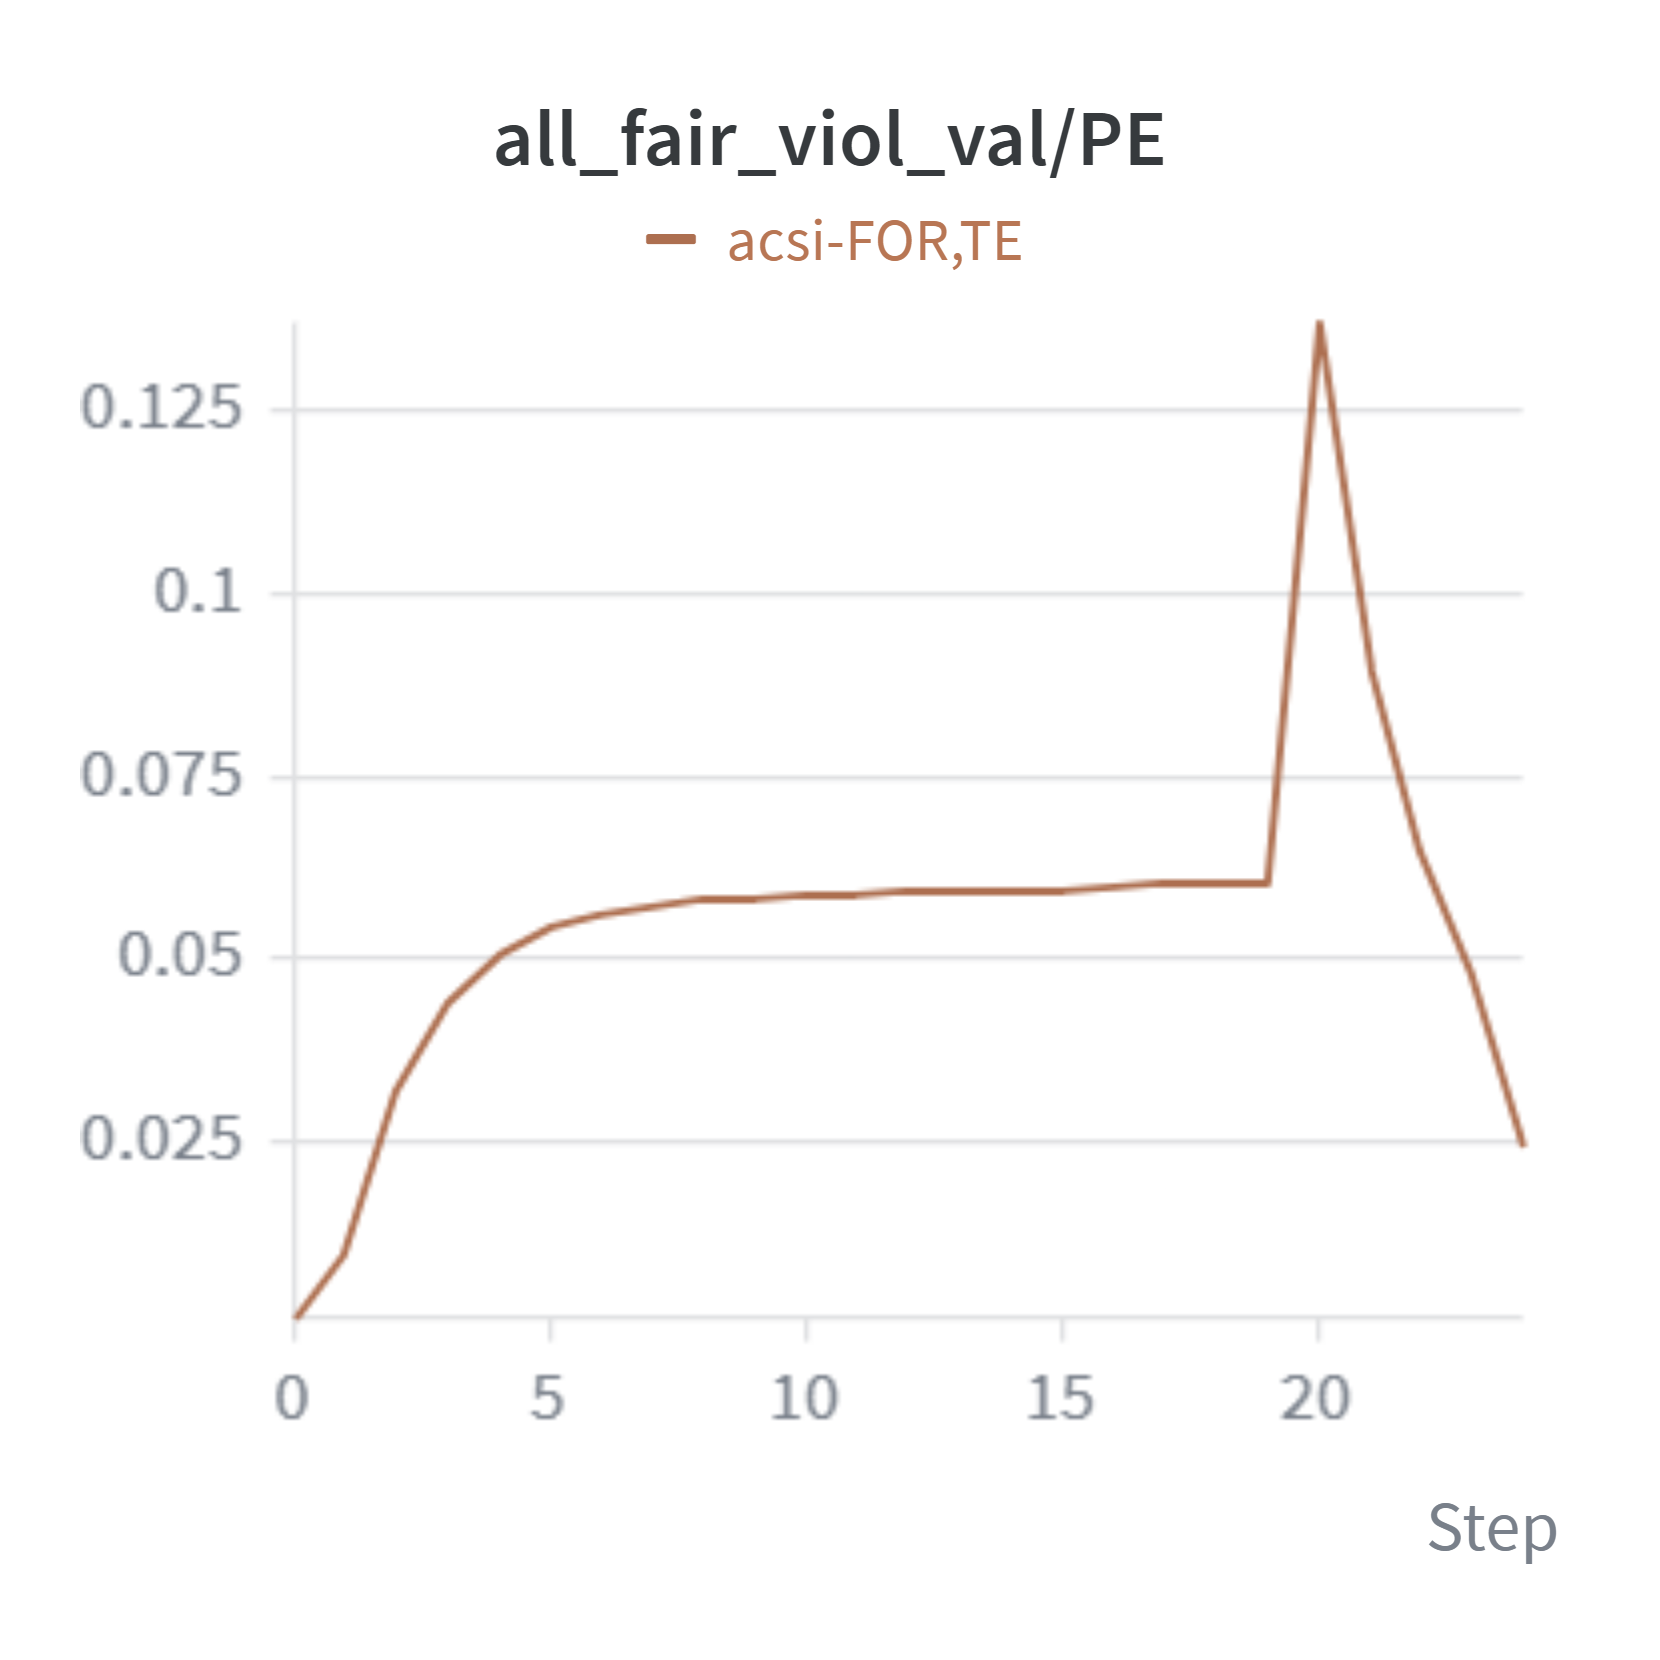
\includegraphics[width=0.45\textwidth]{assets/combined/ACSIncome_FORTE3.png}
    \hfill
    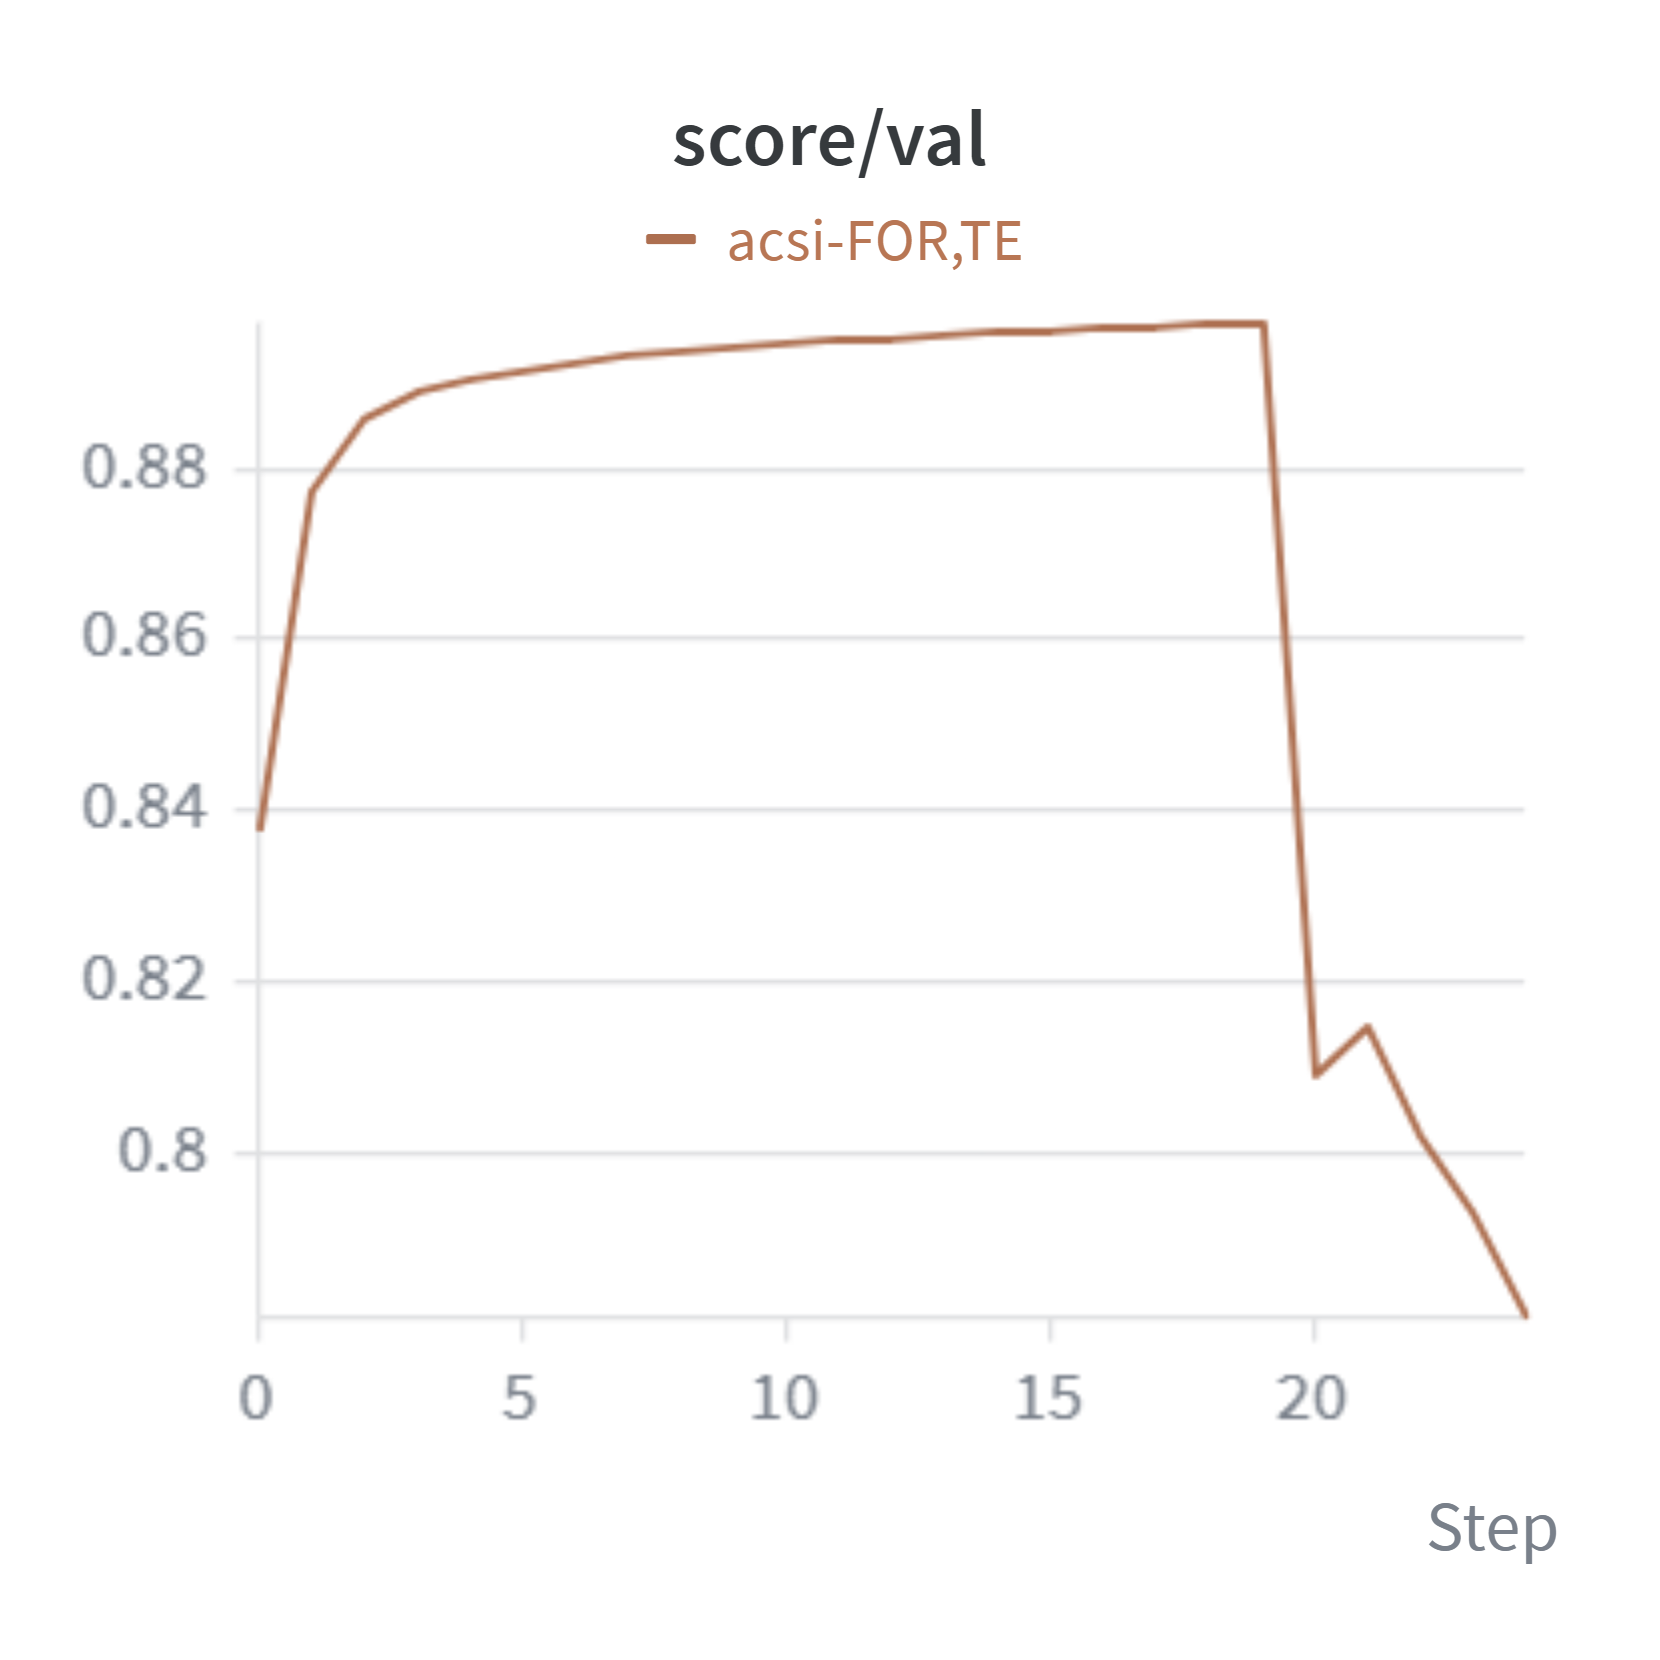
\includegraphics[width=0.45\textwidth]{assets/combined/ACSIncome_FORTE4.png}
    \caption{Validation training curves of FOR-TE constraints with significantly increased strengths. The 20 initial steps are unconstrained afterwards 5 steps are include constraints. Validation violations for FOR, TE, PE are shown and also the validation AUROC.}
    \label{fig:forte}
\end{figure}

\section{Discussion}

The results provide evidence that the theoretically compatible combinations of fairness constraints can also be applied in practice without necessarily resulting in degenerate models. For nearly all evaluated combinations, the relevant fairness metrics could be improved compared with the unconstrained baseline while retaining acceptable predictive performance. This supports the theoretical compatibility analysis of Defrance \& De Bie \cite{max_combinations}.
\todo{TODO: improve discussion}
